\begin{minipage}[l]{0.5\textwidth}
 \begin{exerciseS}[Profilo oscillante]
 L'obiettivo di una prova in galleria è lo studio del campo di moto
  attorno a una pala di elicottero, in particolare attorno alla sezione
  che si trova a metà della lunghezza della pala, $R_v = 6.85\ m$. Il rotore
  dell'elicottero ruota con una velocità angolare $\Omega_v$, tale da
  avere una velocità $U_{tip} = 200 \ m/s$ (per evitare il regime
  supersonico). La corda della pala nella sezione analizzata è
  $c_v = 0.30 \ m$.
 Il modello di galleria a circuito aperto è costituito da una superficie
  alare, incernierata su un asse perpendicolare alla direzione del vento
  di galleria, in corrispondenza dell'asse ``di comando del passo''.
 Sapendo che la massima velocità raggiungibile nell'impianto utilizzato
  è $U_m = 50 \ m/s$, si chiede di determinare:
\begin{itemize}
  \item la corda del modello $c_m$, per ottenere la similitudine in $Re$ e di
    commentare gli effetti di comprimibilità;
  \item la frequenza di oscillazione $\omega_m$ da imporre al profilo per
    simulare il cambio di incidenza dovuti ai comandi di passo collettivo
    e ciclico;
  \item una stima della potenza dell'impianto necessaria a svolgere la prova,
    conoscendo le dimensioni della camera di prova rettangolare, $b = 1.5 \ m$,
    $h = \ 1.0 m$.
\end{itemize}  
 \end{exerciseS}
\hfill
\end{minipage}
\hspace{3mm}
\begin{minipage}[r]{0.5\textwidth}
 \centering
  \includegraphics[width=1.0\textwidth]{./fig/helicopter}
\end{minipage}

\sol

\partone
 Similitudine fluidodinamica. Comando elicottero. Stima potenza galleria del vento.

\parttwo

\begin{itemize}
\item
Per ottenere la similitudine in $Re$, è necessario uguagliare i numeri di Reynolds 
 ottenuti con le grandezze dimensionali caratteristiche del problema.
 La lunghezza di riferimento è la corda. La velocità di riferimento è la velocità
 che investe il profilo della pala considerato; nella prova di galleria è la velocità
 di galleria $U_m$, nella realtà è la velocità relativa dovuta alla rotazione della
 pala (alla quale deve essere sovrapposto il moto dell'elicottero, in caso di avanzamento,
 qui ipotizzato nullo): $U_v = \Omega \ R_v/2 = U_{tip}/2$. Il fluido è sempre aria.
\begin{equation}
  \dfrac{U_v c_v}{\nu} =   \dfrac{U_m c_m}{\nu} \quad \Rightarrow \quad
  c_m = c_v \dfrac{U_{tip}}{2 \ U_m} = 0.60 \ m
\end{equation}
 In questo esempio, per avere similitudine in $Re$ serve un modello con una
 corda maggiore della corda reale.

Gli effetti di comprimibilità possono essere valutati calcolando il numero di Mach.
 Il numero di Mach per la sezione di pala considerata nella realtà è 
 $M_v \approx 100 / 340 \approx 0.3$, limite convenzionale per potere trascurare gli
 effetti di comprimibilità. Per la prova in galleria $M_m \approx 0.15$.

\item
Il comando di passo ciclico è periodico e armonico con frequenza 
 $\Omega_v = U_{tip}/R_v = 29.19 \ s^{-1}$. Per essere in similitudine con la realtà
 è necessario avere uguaglianza dei numeri di Strouhal (o \textit{frequenze ridotte},
 indicate da strutturisti e aeroelastici con $k$).
\begin{equation}
 \dfrac{\Omega c_v}{U_v} = \dfrac{\omega_m c_m}{U_m} \quad \Rightarrow \quad
  \omega_m = \Omega \dfrac{c_v}{c_m}\dfrac{U_m}{U_v} = \Omega \left(\dfrac{U_m}{U_v}\right)^2
\end{equation}

\item
In un impianto a galleria aperta si può ricavare la formula per la stima della potenza
 necessaria da un bilancio integrale di energia cinetica
\begin{equation}
 P \approx \dfrac{1}{2}\rho U^3 A \ .
\end{equation}
\end{itemize}



